\chapter{Introduction Générale}
Chaque rapport doit commencer par une introduction générale dans laquelle le contexte du projet est clairement expliqué. Cette introduction devrait également inclure l'objectif du projet et le plan du reste du rapport. Cette introduction ne devrait pas dépasser 2 pages. Soyez concis et clair, et écrivez uniquement ce qui est nécessaire à écrire.

\section{Introduction}
L'apprentissage automatique, également connu sous le nom de « machine Learning »,est une sous-discipline de l'intelligence artificielle (IA) qui se concentre sur le développement de techniques permettant aux systèmes informatiques d'apprendre à partir de données, sans être explicitement programmés. Plutôt que de suivre des instructions programmées, les algorithmes d'apprentissage automatique utilisent des modèles statistiques pour identifier des motifs et tirer des conclusions à partir des données d’entrée. \cite{1}
Dans ce chapitre, nous nous intéressons aux techniques d’apprentissage automatique. Dans une première partie, nous présentons les deux types d’apprentissage automatique :
L’apprentissage supervisé et l’apprentissage non supervisé. Ensuite, nous présentons les méthodes de classification supervisées qui ont été utilisées dans notre étude notamment, SVM, Logistique Régression, Arbres de décision et K-plus proche voisins et a la fin de chapitre, nous vous présentons Définition de Deep Learning et Modèles du Deep Learning(CNN , RNN et LSTM).

\section{L'apprentissage profondeur (Deep Learning) }
L’intérêt de l’apprentissage automatique a augmenté au cours de la dernière décennie, pour tout le discours sur l’apprentissage automatique, il y a beaucoup de conflits entre ce que la machine peut faire et ce que nous souhaitons.
 D’une façon générale, l'apprentissage automatique est un type d'intelligence artificielle (IA), c’est une science qui permet aux ordinateurs d'apprendre sans être explicitement programmés « Arthur Samuel, 1959 ». Plus précisément, l'apprentissage automatique fait référence au développement, l'analyse et l'implémentation de méthodes qui permettent à une machine (au sens large) d'évoluer et de remplir des tâches associées à une intelligence artificielle grâce à un processus d'apprentissage. Cet apprentissage permet d'avoir un système qui s'optimise en fonction de l'environnement, les expériences et les résultats observés.
Dans le domaine médicale, l’apprentissage automatique a été conçu pour réaliser l'analyse de données médicales, surtout lorsque l'évolution numérique a fourni des moyens (capteurs) peu coûteux permettant de recueillir et de stocker des informations importantes liées aux patients et maladies. Par exemple, les algorithmes d'apprentissage sont utiles au médecin lors du diagnostic des patients, afin d'améliorer la vitesse, la précision et la fiabilité de son diagnostic.

\section{Types d’Apprentissage Automatique  }
Il existe fondamentalement quatre types d’apprentissage automatique : Supervisé, semi-supervisé et non-supervisé et Apprentissage par renforcement. 
Dans notre étude, nous utilisons l’apprentissage supervisé pour construite des modèles pour la prédiction des maladies.
Dans la suite de cette section, nous allons présenter les deux types d’apprentissage les plus utilisés qui sont l’apprentissage supervisé et apprentissage non supervisé.
\begin{figure}[h]
    \centering
    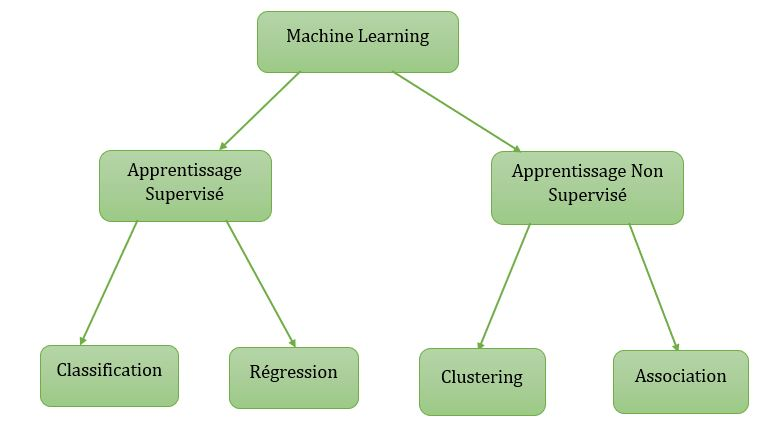
\includegraphics[scale=0.3]{Images/Chapter1/sup unsup.JPG}
    \caption{Les différentes méthodes d'apprentissage automatique.}
    \label{fig:01}
    \end{figure}
    \subsection{Apprentissage Supervisé }
    Dans l'apprentissage supervisé, l'ordinateur est fourni avec des exemples d'entrées qui sont étiquetés avec les sorties souhaitées. Le but de cette méthode est que l'algorithme puisse « apprendre » en comparant sa sortie réelle avec les sorties « apprises » pour trouver des erreurs et modifier le modèle en conséquence. 
L'objectif des algorithmes d'apprentissage supervisé est d'apprendre une fonction qui mappe les vecteurs de caractéristiques (entrées) aux étiquettes (sortie), sur la base d'exemples de paires entrée-sortie.  

Comme il est illustré dans la Figure 1 l’apprentissage supervisé peut être utilisé pour deux types de tâches principales : la classification et la régression. 
Les algorithmes de classification cherchent à prédire la classe ou la catégorie à laquelle appartient une donnée d'entrée tandis que les algorithmes de régression servent à prédire une valeur numérique continue à partir de variables d'entrée. Dans ce travail, nous nous intéressons aux méthodes de classification.
\subsection{1.3.2.	Apprentissage Non-Supervisé }
Dans l'apprentissage non supervisé, les données sont non étiquetées, de sorte que l'algorithme d'apprentissage trouve tout seul des points communs parmi ses données d'entrée. Les données non étiquetées étant plus abondantes que les données étiquetées, les méthodes d'apprentissage automatique qui facilitent l'apprentissage non supervisé sont particulièrement utiles.
L'objectif de l'apprentissage non supervisé peut être aussi simple que de découvrir des modèles cachés dans un ensemble de données.
Les plus fréquents problèmes connus dans ce type sont :
\begin{itemize}
    \item Le clustering qui consiste à regrouper un ensemble d’éléments hétérogènes sous forme de sous-groupes homogènes.
    \item La réduction de dimension qui consiste à prendre des données dans un espace de grande dimension, et à les remplacer par des données dans un espace de plus petite dimension sans perdre la variance \cite{2}
\end{itemize}
\section{Algorithmes de Classification }
Dans cette partie, nous présentons les algorithmes de classification \cite{3} \cite{4} \cite{5}.
\subsection{Les k plus proches voisins (KNN)}
L’algorithme des K-Nearest Neighbors (KNN) (K plus proches voisins) est un algorithme de classification supervisé. Chaque observation de l’ensemble d’apprentissage est représentée par un point dans un espace à n dimensions ou n est le nombre de variables prédictives. Pour prédire la classe d’une observation, on cherche les k points les plus proches de cet exemple. La classe de la variable cible, est celle qui est la plus représentée parmi les k plus proches voisins. Il existe des variantes de l’algorithme ou on pondère les k observations en fonction de leur distance à l’exemple dont on veut classer \cite{6}, les observations les plus éloignées de notre exemple seront considérées comme moins importantes.
\begin{figure}[h]
    \centering
    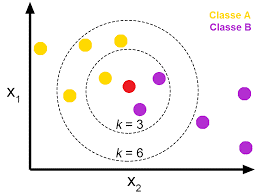
\includegraphics[scale=0.3]{Images/Chapter1/knn.png}
    \caption{Pour k = 3 la classe majoritaire du point central est la classe B, mais si on change la valeur du voisinage k = 6 la classe majoritaire devient la classe A}
    \label{fig:02}
    \end{figure}
    \begin{itemize}
        \item \textbf{Avantages }
        \begin{itemize}
            \item Simple à concevoir .
        \end{itemize}
    
        \item \textbf{Inconvénients}
        \begin{itemize}
            \item Sensible aux bruits.
            \item Pour un nombre de variable prédictives très grands, le calcul de la distance devient très coûteux.
        \end{itemize}
    \end{itemize}
\subsection{k-means}
L’algorithme des k-moyennes (k-means) est un algorithme non supervisé. Chaque observation est représentée par un point dans un espace à n dimensions ou n est le nombre de variables descriptives.
À partir d’un ensemble d’apprentissage de M observations[X^{(1)}, \ldots, X^{(M)}] cet algorithme va repartir ces observations en k clusters de manière à ce que la distance euclidienne qui sépare les points au centre de gravité du groupe auquel ils sont affectés soit minimale. Les étapes de l’algorithme sont 
\begin{enumerate}
    \item Choisir k points qui représentent la position moyenne des clusters.
    \item répéter jusqu’à stabilisation des points centraux :
    \begin{itemize}
        \item affecter chacun des M points au plus proche des k points centraux .
        \item mettre à jour les points centraux en calculant les centres de gravité des k cluster .
    \end{itemize}
\end{enumerate}
\begin{itemize}
    \item \textbf{Avantages}
    \begin{itemize}
        \item implémentable pour des grands volumes de données.
    \end{itemize}
    \item \textbf{Inconvénients}
    \begin{itemize}
        \item Le choix du paramètre k n’est pas découvert mais choisi par l’utilisateur.
        \item La solution dépend des k centre de gravité choisi lors de l’initialisation.
    \end{itemize}
    \begin{figure}[h]
        \centering
        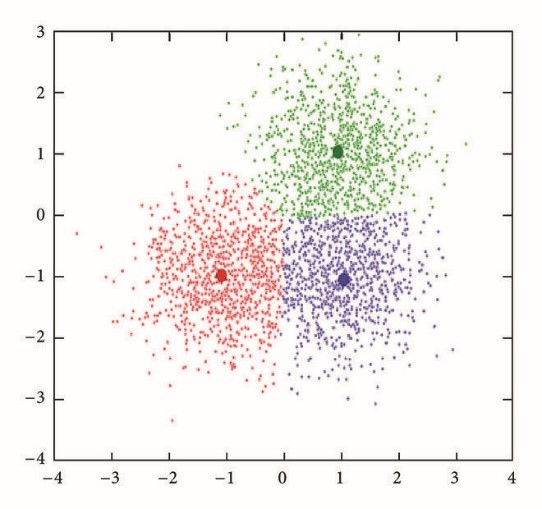
\includegraphics[scale=0.3]{Images/Chapter1/kmeans.jpg}
        \caption{L’algorithme k-means regroupe les données en k cluster, ici k = 3. Les centres de gravité sont représentés par de petit cercle}
        \label{fig:03}
        \end{figure}    
\end{itemize}
\subsection{Régression Logistique}
L'analyse de régression est souvent utilisée pour faire des prédictions, comprendre les variables indépendantes par rapport à la variable dépendante et étudier la forme de leur relation.
Dans des circonstances limitées, l'analyse de régression peut être utilisée pour déduire la relation causale entre la variable indépendante et la variable dépendante.
La régression est un algorithme robuste lorsqu'il s'agit de classer des ensembles de problèmes, et a une fonction logistique (fonction sigmoïde) au cœur de celui-ci. Dans cet algorithme, les valeurs d'entrée sont combinées en fonction de coefficients ou de poids pour donner les valeurs de sortie/prédites. \cite{7}.
\begin{figure}[h]
    \centering
    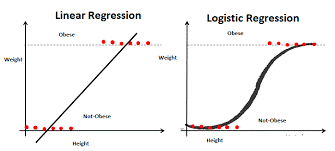
\includegraphics[scale=0.3]{Images/Chapter1/regre.png}
    \caption{La différence entre la régression logistique et la régression linéaire.}
    \label{fig:04}
    \end{figure} 
    \begin{itemize}
        \item \textbf{Avantages}
        \begin{itemize}
            \item Ses résultats sont faciles à interpréter.
        \end{itemize}
        \item \textbf{Inconvénients}
        \begin{itemize}
            \item La phase d’apprentissage peut être longue car l’optimisation des coefficients est complexe.
            \item Sa linéarité empêche la prise en compte des interactions entre les variables.
        \end{itemize}
        \subsection{Machine à Vecteurs de Supports (S V M)}
        Support Vector Machine (SVM) est l’un des algorithmes d’apprentissage supervisé les plus populaires, utilisé pour les problèmes de classification et de régression. 
        Cependant, il est principalement utilisé pour les problèmes de classification dans l’apprentissage automatique. Le but de l’algorithme SVM est de créer la meilleure ligne ou limite de décision qui peut séparer l’espace à n dimensions en classes afin que nous puissions facilement mettre le nouveau point de données dans la bonne classe à l’avenir.
        
        \begin{figure}[h]
            \centering
            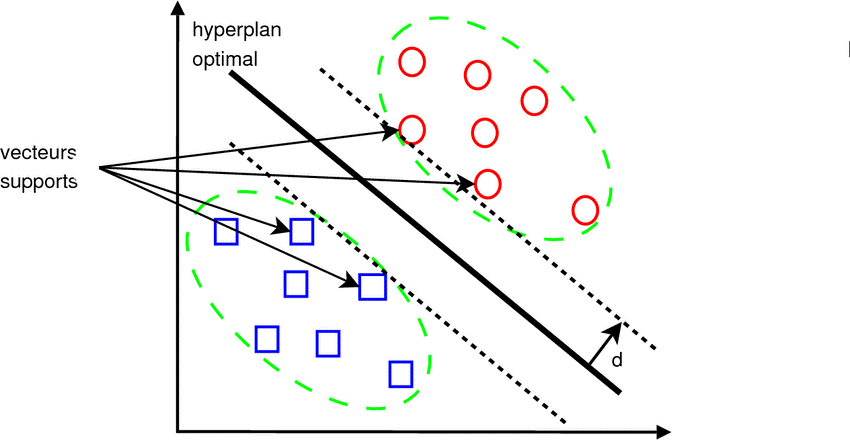
\includegraphics[scale=0.3]{Images/Chapter1/svm.png}
            \caption{Les vecteurs de support, hyperplan et la marge.}
            \label{fig:05}
            \end{figure} 
            \begin{itemize}
                \item \textbf{Avantages}
                \begin{itemize}
                    \item Il permet de traiter des problèmes de classification non linéaire complexe.
                    \item Les SVM constituent une alternative aux réseaux de neurones car plus faciles à entraîner.
                \end{itemize}
                \item \textbf{Inconvénients}
                \begin{itemize}
                    \item Les SVM sont souvent moins performants que les forets aléatoires.
                \end{itemize}
   \section{L'apprentissage profondeurd (Deep Learning)}
   Le Deep Learning ou apprentissage profond est un type d'intelligence artificielle dérivé du machine Learning (apprentissage automatique) où la machine est capable d'apprendre par elle-même, contrairement à la programmation où elle se contente d'exécuter à la lettre des règles prédéterminées.
   Le deep learning est une sous-discipline de l'intelligence artificielle qui se concentre sur l'apprentissage automatique de représentations de données à plusieurs niveaux, souvent basées sur des architectures de réseaux de neurones artificiels composés de nombreuses couches (d'où le terme "profond") permettant de modéliser et d'abstraire des données complexes et de capturer des structures hiérarchiques. Ces réseaux sont entraînés sur de grandes quantités de données à l'aide d'algorithmes d'optimisation tels que la rétropropagation, afin d'apprendre à extraire automatiquement des caractéristiques pertinentes des données \cite{8}.
   \section{Modéles du Deep Learning}
   On va présenter dans cette section les modèles de deep learning utilisés dans notre proposition (à savoir les CNN, RNN et les LSTM).
   \subsection{Réseau de neurones à convolution (CNN)}
   Le nom « Réseau de neurones à convolution » indique que le réseau emploi une opération mathématique appelée la convolution.
 Les réseaux de convolution sont un type spécialisé de réseaux neuronaux qui utilisent la convolution à la place de la multiplication matricielle générale dans au moins une de leurs couches.
Les CNN sont l’un des meilleurs algorithmes d’apprentissage pour faire l’opération de convolution qui aide à l’extraction de fonctionnalités utiles à partir de points de données corrélés localement. La sortie des noyaux convolutifs est ensuite affectée à l’unité de traitement non linéaire (fonction d’activation), qui non seulement aide à apprendre les abstractions, mais intègre également la non-linéarité dans l’espace des fonctionnalités.
La topologie de CNN est divisée en plusieurs étapes d’apprentissage composées d’une combinaison des couches convolutives, des unités de traitement non linéaires et des couches de sous-échantillonnage (Jarrett et al., 2009) \cite{9}.
\begin{figure}[h]
    \centering
    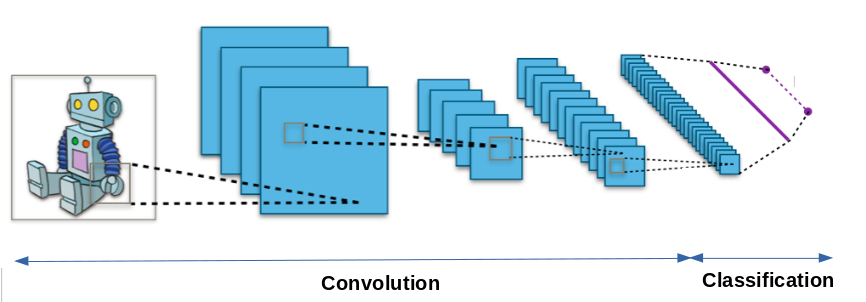
\includegraphics[scale=0.3]{Images/Chapter1/cnn.png}
    \caption{Réseau de neurones avec de nombreuses couches convolutives.}
    \label{fig:06}
    \end{figure}
    \subsection{Réseaux Neuronaux Récurrents (RNN)}
    Les Réseaux Neuronaux Récurrents (RNN) sont une variante très importante de réseaux neuronaux lourdement utilisés dans le traitement de langue naturelle. 
    Ils sont appelés récurrents car ils effectuent la même tâche pour chaque élément d'une séquence, la sortie dépendant des calculs précédents. 
    Une autre façon de penser aux RNN est qu'ils ont une « mémoire » qui capture des informations sur ce qui a été calculé jusqu'à présent. En théorie, les RNN peuvent utiliser des informations dans des séquences arbitrairement longues, mais en pratique, ils se limitent à ne regarder que quelques étapes en arrière.
     Les RNNs sont une classe de réseaux de neurones qui permettent aux prédictions antérieures d'être utilisées comme entrées, par le biais d'états cachés.    
 \begin{figure}[h]
     \centering
     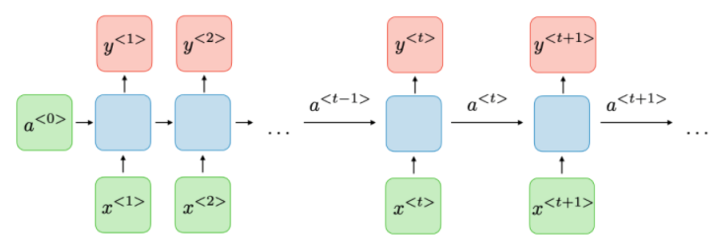
\includegraphics[scale=0.3]{Images/Chapter1/rnn.png}
     \caption{Architecture de RNN.}
     \label{fig:07}
     \end{figure}
     \subsection{Réseaux Long Short-Term Memory (LSTM)}
     Ce sont un type spécial de RNN, capable d'apprendre les dépendances à long terme. 
     Ils ont été introduits par (Hochreiter et Schmidhuber, 1997), et ont été affinés et popularisés par de nombreuses personnes dans les travaux suivants. Ils fonctionnent extrêmement bien sur une grande variété de problèmes et sont maintenant largement utilisés.
     Les LSTM sont explicitement conçus pour éviter le problème de dépendance à long terme. Se souvenir des informations pendant de longues périodes est pratiquement leur comportement par défaut, pas quelque chose qu'ils ont du mal à apprendre !
     Tous les réseaux de neurones récurrents ont la forme d'une chaîne de modules répétitifs de réseau de neurones \cite{10}.
     Les LSTM ont des mécanismes intégrés qui leur permettent de mémoriser et d'oublier sélectivement des informations au fil du temps, ce qui les rend plus efficaces pour traiter des séquences à long terme.
     Ils sont couramment utilisés dans des applications nécessitant une compréhension à long terme, comme la traduction automatique, la génération de texte et d'autres tâches séquentielles complexes
         
 \begin{figure}[h]
     \centering
     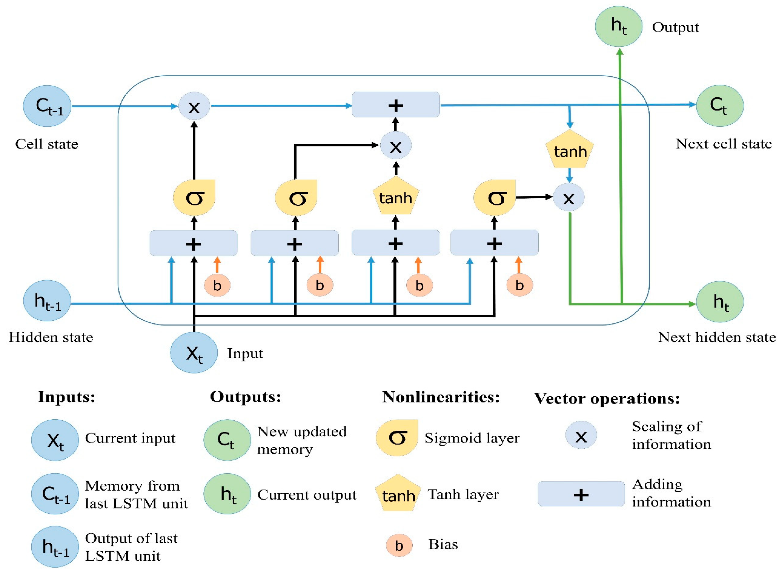
\includegraphics[scale=0.3]{Images/Chapter1/ltsm.png}
     \caption{: Le module répétitif dans un LSTM.}
     \label{fig:08}
     \end{figure}
     \section{Conclusion }
     Dans ce chapitre, nous avons présenté les algorithmes d'apprentissage automatique. Après avoir présenté les deux principaux types d’apprentissage automatique, une description détaillée de chaque méthode de classification a été fournie, expliquant le principe de fonctionnement de chaque méthode ainsi que ses avantages et inconvénients.
Nous avons également identifié les techniques d'apprentissage profond et les bases de leur travail, qui constitueront la base de nos prochains travaux.
   Le chapitre suivant présente quelques travaux connexes où les méthodes d'apprentissage automatique ont été appliquées dans le domaine de la santé.